%!TEX root = ../main.tex

% \subsection{Number of Storms}

% \par
% Much of this section will be devoted to explaining the mathematics and statistical methods for answering my questions. Implementation details will 

% \par
% I will attempt to find the distributions which best fit the data on number of storms based on various loss functions.
% Note that the number of landfalling storms is discrete.
% The distributions I plan to examine include
% \begin{itemize}
% 	\item Poisson
% 	\item Negative Binomial
% \end{itemize}
% I also plan to compare to a non-parametric distribution.
% For loss functions, I will examine common examples such as the 0-1 and quadratic loss functions, as well as defining some specific loss functions that make sense in the context of hurricanes.

% \subsection{Predicting a Storm's Outcome}

% \par
% In order to predict whether a storm will make landfall, we have several methods.
% One method we will try is using the various similarity metrics presented by the paper I mention in related work to find the closest-match hurricane or the $n$-closest-matches (based on limited data from the start of the hurricane).
% Another method will be to learn probability distributions based on certain conditions of the start of the hurricane, such as location or origin and rate of intensification in size, wind speed, and other characteristics.

% \par
% In order to predict the conditions of a storm's landfall, I intend to approximate the various aspects (max wind speed, atmospheric pressure) with several continuous distributions, as well as a non-parametric distribution.
% I also plan to model multiple conditions simultaneously with multivariate distributions (such as a mixture of Gaussians) -- we know there should be a clear correlation between max wind speed and atmospheric pressure, and a multivariate distribution should better reflect this than independent single-variable distributions.

% \subsection{Outlier Analysis}

% \par
% In this section, I plan to examine the frequency of outliers in several aspects of the hurricane, including the maximum extend of certain wind speeds (informally, the ``size'' of the hurricane), and maximum wind speed.
% I will perform this analysis by fitting several continuous distributions, such as the Cauchy and Normal distributions, to the data, and examining which fit better.
% Based on this, I can consider how large the tail of the distribution is, and hence how likely rare storms are.

\par
There are four parts to the methodology.
First, I discuss the time series similarity metrics presented by \cite{ho2015manifold} in their paper \textit{Manifold Learning for Multivariate Variable-Length Sequences With an Application to Similarity Search}.
Then, I explain how the metrics are used to perform dimensionality reduction on the hurricane tracks.
Next, I present the local linear extension to Nadaraya-Watson kernel regression.
Finally, I explain how to use the learned model to predict whether a hurricane will make landfall.

\subsection{Time Series Similarity Metrics}

\newcommand{\LCSS}{\operatorname{LCSS}}
\newcommand{\SLC}{\operatorname{SLC}}

\par
In order to compare two hurricanes, we model their tracks as arbitrary-length multivariate spatiotemporal data sequences.
Consider two hurricanes with track lengths $r$ and $s$. Then their data sequences are
\[
	A=[(t_{A,1},x_{A,1},y_{A,1}),\ldots,(t_{A,r},x_{A,r},y_{A,r})]
\]
and
\[
	B=[(t_{B,1},x_{B,1},y_{B,1}),\ldots,(t_{B,r},x_{B,r},y_{B,r})]
\]
(respectively).
The $t_{*}$ are translated so that $t_{*,1}=0$, and the $x$ and $y$ coordinates correspond to longitude and latitude (respectively).

\par
I now present slightly modified versions of two similarity metrics used in the paper.
There are parameters $\delta,\varepsilon>0$, where $\delta$ controls the temporal similarity range, and $\varepsilon$ controls the distance similarity range.
Let $\mathscr{L}(A)$ give the length of $A$, and let $\mathscr{R}(A)$ return all but the last term of the time series $A$.
Indexing by $-1$ is taken to mean accessing the last element in a list.
\par
Define
\begin{equation}
	M_{1}(A,B,\delta,\varepsilon)=\frac{\LCSS(A,B,\delta,\varepsilon)}{\min\set{\mathscr{L}(A),\mathscr{L}(B)}}
	\label{eq:m1}
\end{equation}
and
\begin{equation}
	M_{2}(A,B,\delta,\varepsilon)=\frac{\SLC(A,B,\delta,\varepsilon)}{\min\set{\mathscr{L}(A),\mathscr{L}(B)}}
	\label{eq:m2}
\end{equation}
$\LCSS(A,B,\delta,\varepsilon)$ is the approximate longest common subsequence, and $\SLC(A,B,\delta,\varepsilon)$ is the soft longest common subsequence.
I explicitly write out their equations in Figure~\ref{fig:subsequences}, and implement them using bottom-up dynamic programming.

\begin{figure*}
	\centering
	\begin{equation}
		\LCSS(A,B,\delta,\varepsilon)=\left\{\begin{array}{ll}
			0 & \mathscr{L}(A)=0\;\ptxt{or}\;\mathscr{L}(B)=0\\
			1+\LCSS(\mathscr{R}(A),\mathscr{R}(B)) & \abs{t_{A,-1}-t_{B,-1}}<\delta\;\ptxt{and}\;\\
			& \norm{(x_{A,-1},y_{A,-1})-(x_{B,-1},y_{B,-1})}_{2}<\varepsilon\\
			\max\left\{\LCSS(\mathscr{R}(A),B,\delta,\varepsilon),\right.\\
			\phantom{\max\left\{\right.}\!\!\left.\LCSS(A,\mathscr{R}(B),\delta,\varepsilon)\right\} & \ptxt{otherwise}
		\end{array}\right.
		\label{eq:lcss}
	\end{equation}
	\begin{equation}
		\SLC(A,B,\delta,\varepsilon)=\left\{\begin{array}{ll}
			0 & \mathscr{L}(A)=0\;\ptxt{or}\;\mathscr{L}(B)=0\\
			C+\SLC(\mathscr{R}(A),\mathscr{R}(B)) & \abs{t_{A,-1}-t_{B,-1}}<\delta\;\ptxt{and}\;\\
			& \norm{(x_{A,-1},y_{A,-1})-(x_{B,-1},y_{B,-1})}_{2}<\varepsilon\\
			\max\left\{\SLC(\mathscr{R}(A),B,\delta,\varepsilon),\right.\\
			\phantom{\max\left\{\right.}\!\!\left.\SLC(A,\mathscr{R}(B),\delta,\varepsilon)\right\} & \ptxt{otherwise}
		\end{array}\right.
		\label{eq:slc}
	\end{equation}
	\begin{equation}
		C=\min\set{1,1-\frac{\varepsilon-\norm{(x_{A,-1},y_{A,-1})-(x_{B,-1},y_{B,-1})}_{2}}{\varepsilon}}
		\label{eq:slc_c}
	\end{equation}
	\caption{Equations for $\LCSS$ and $\SLC$, used in computing the similarity between spatiotemporal data sequences. Note the usage of Eq~(\ref{eq:slc_c}) in the computation of Eq~(\ref{eq:slc}).}
	\label{fig:subsequences}
\end{figure*}

\begin{figure*}
	\centering
	\begin{subfigure}[t]{0.45\textwidth}
		\centering
		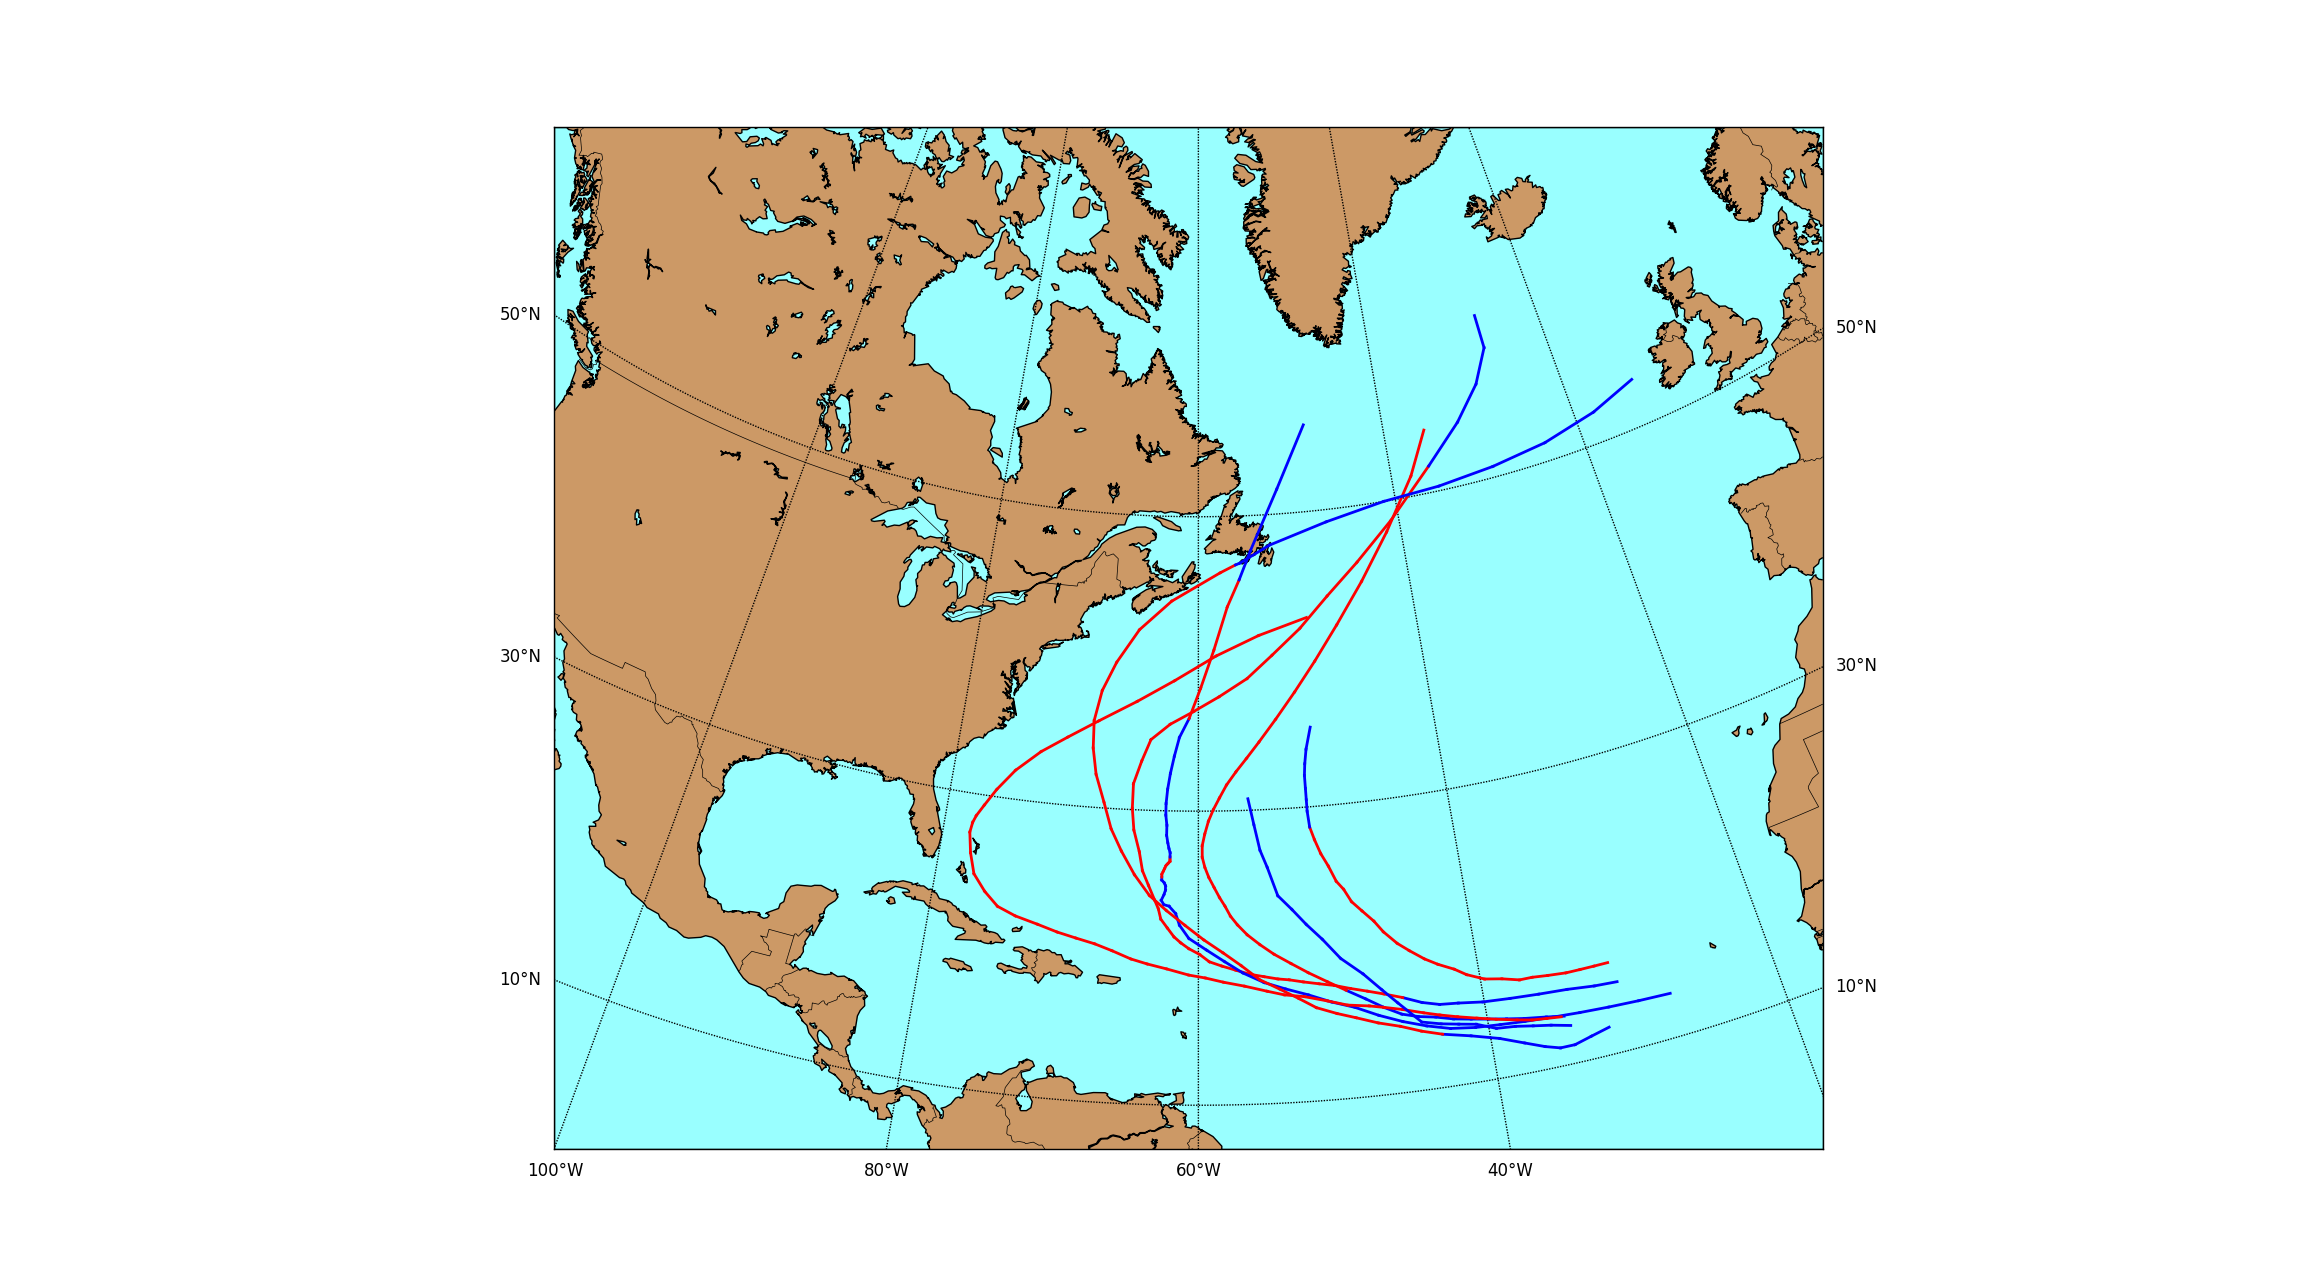
\includegraphics[width=\linewidth, trim=350 50 300 50, clip]{images/similar_hurricanes_1.png}
	\end{subfigure}
	\begin{subfigure}[t]{0.45\textwidth}
		\centering
		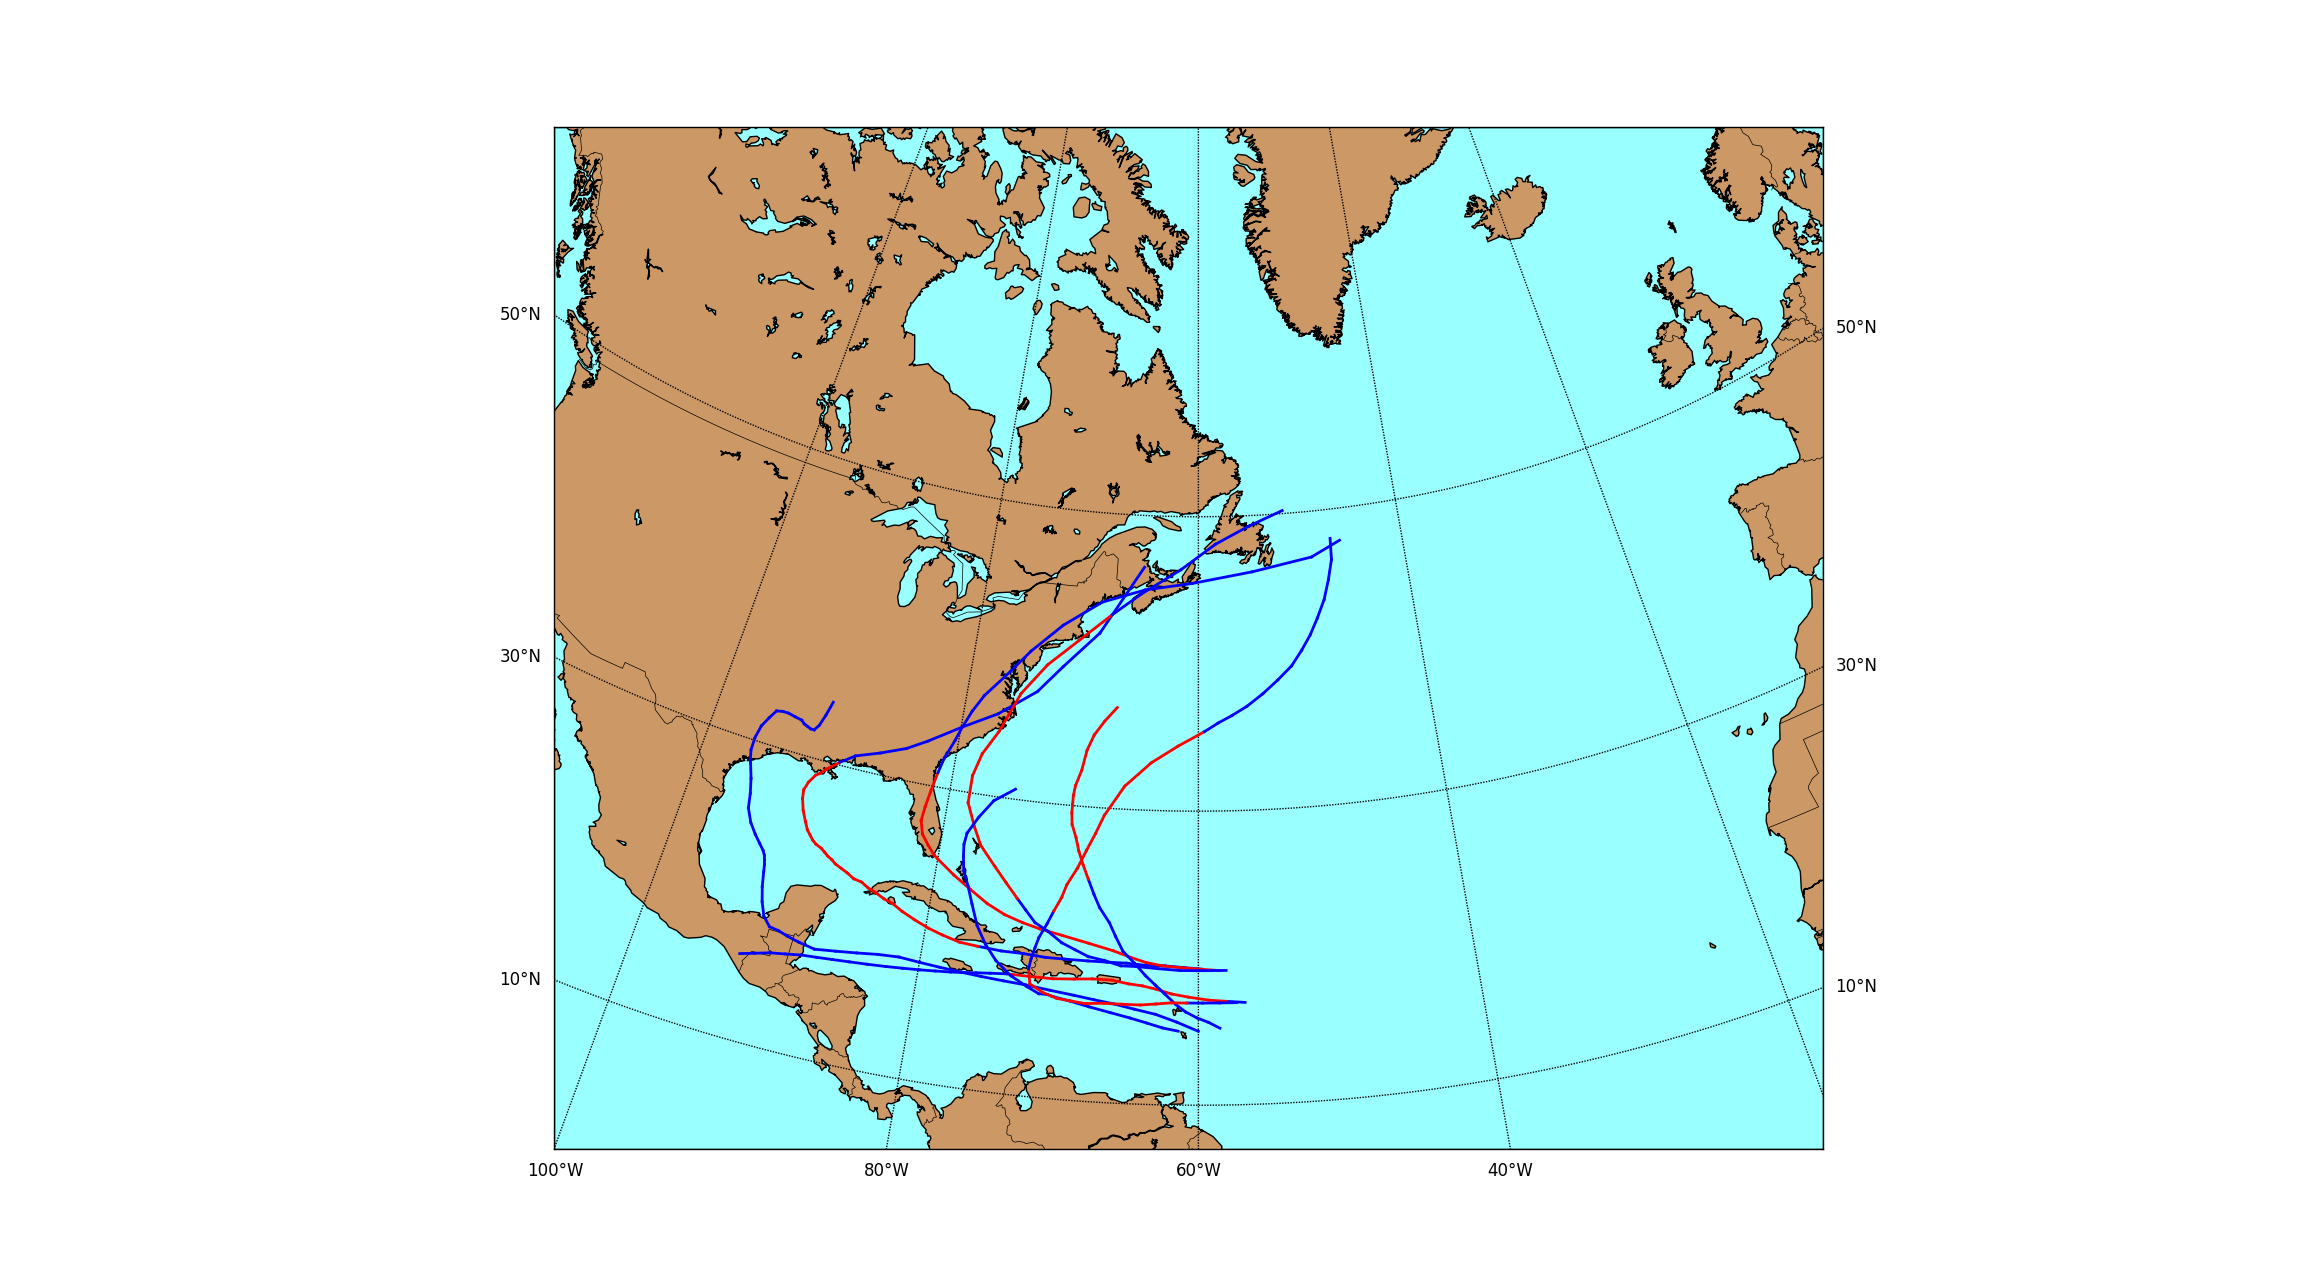
\includegraphics[width=\linewidth, trim=350 50 300 50, clip]{images/similar_hurricanes_5.png}
	\end{subfigure}
	\break
	\begin{subfigure}[t]{0.45\textwidth}
		\centering
		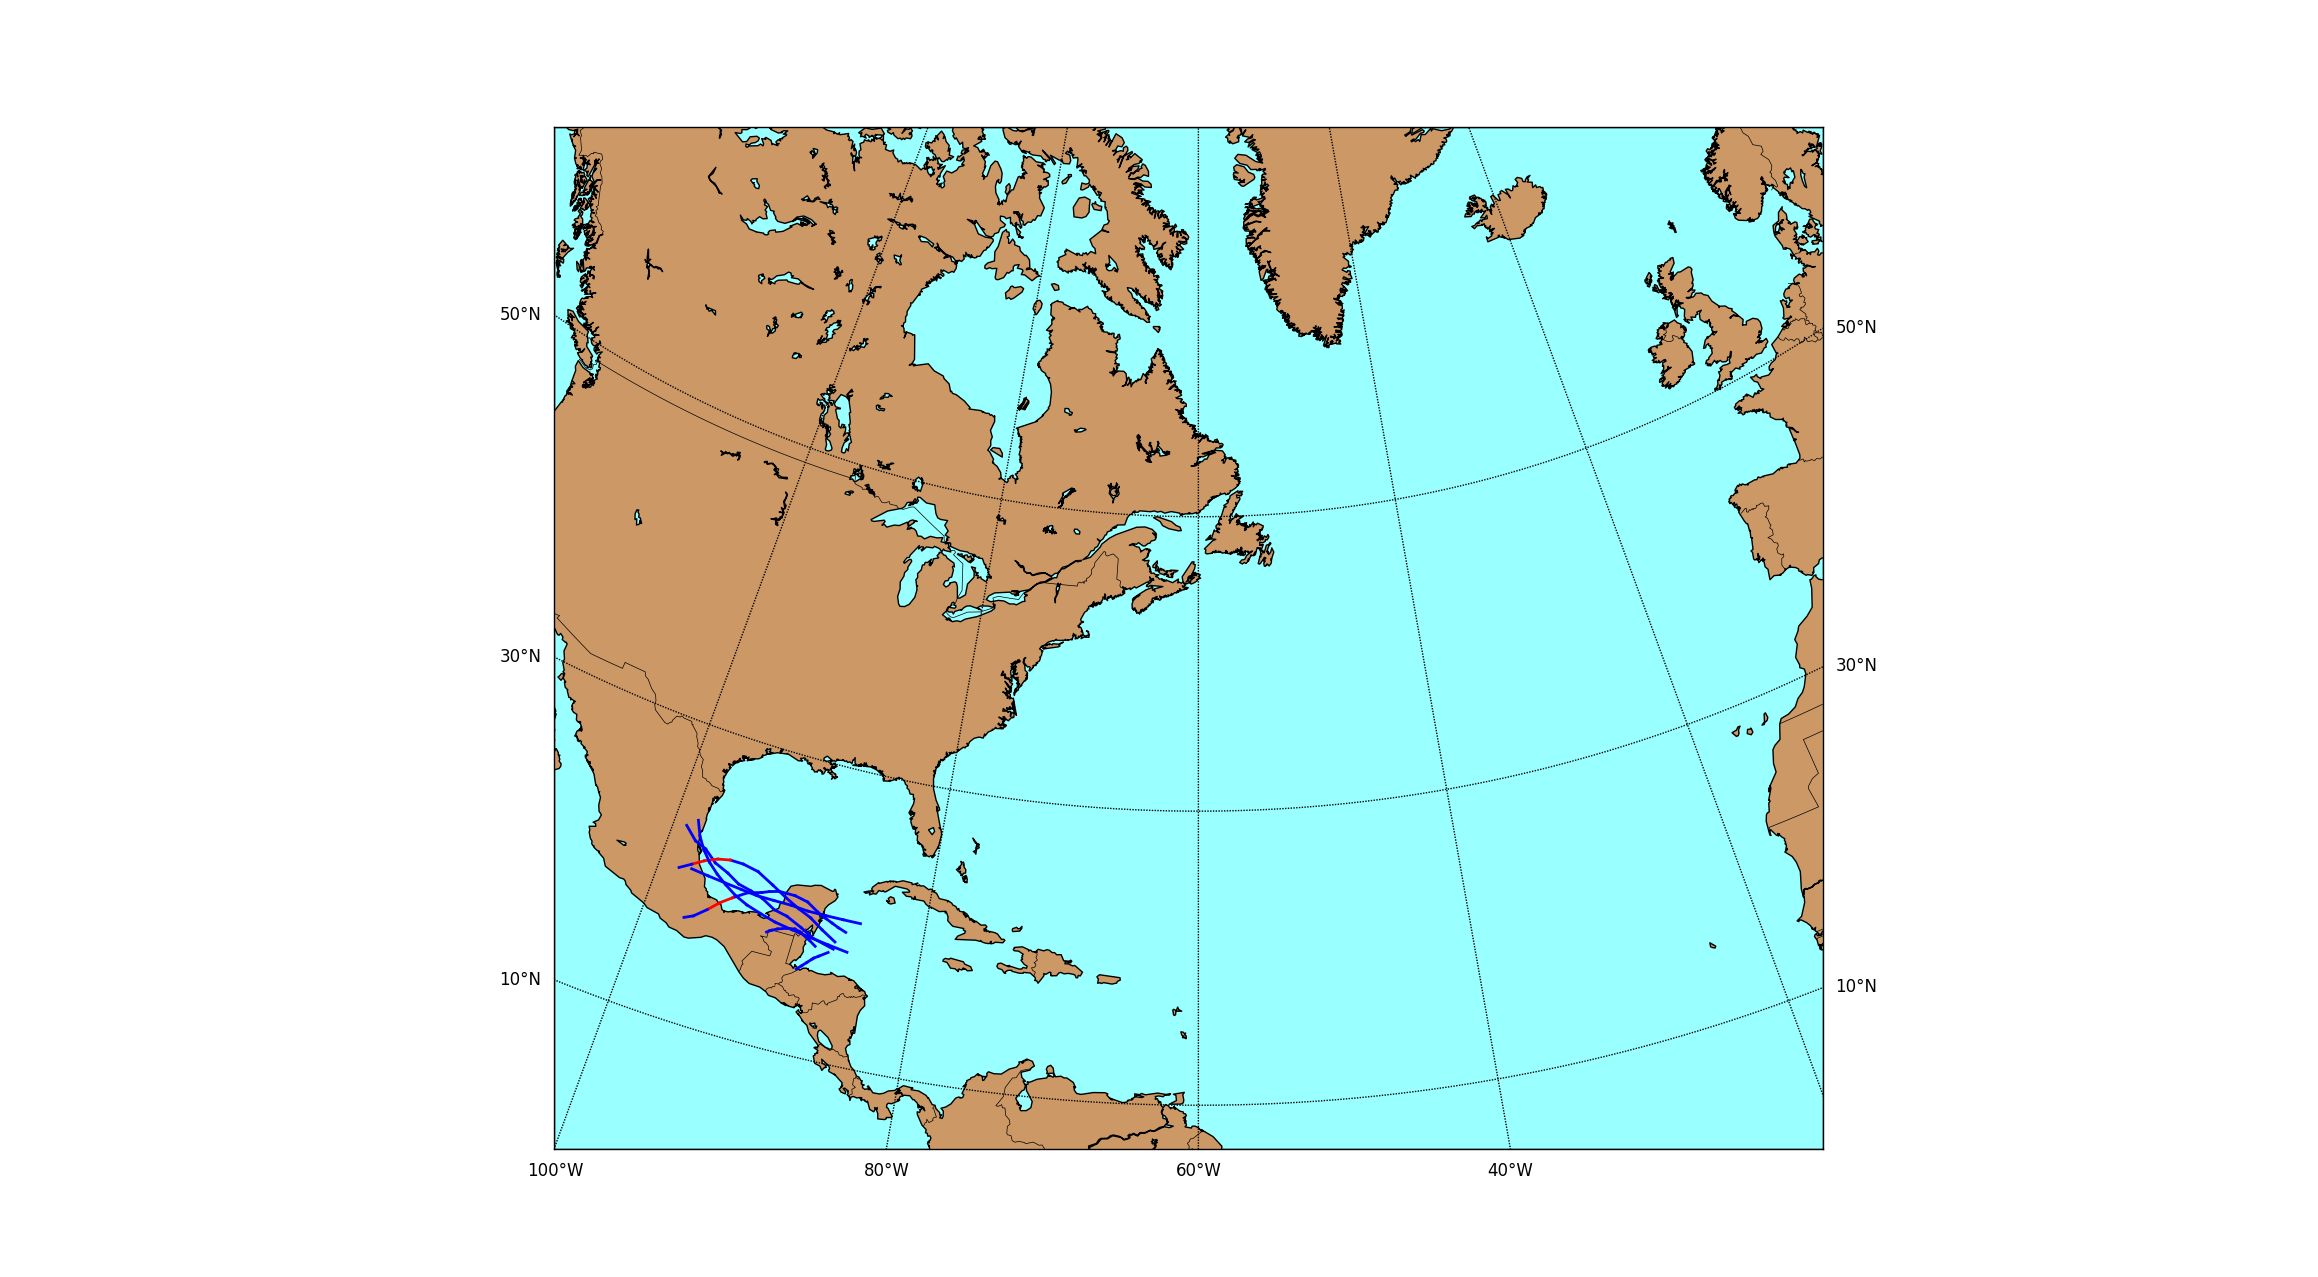
\includegraphics[width=\linewidth, trim=350 50 300 50, clip]{images/similar_hurricanes_3.png}
	\end{subfigure}
	\begin{subfigure}[t]{0.45\textwidth}
		\centering
		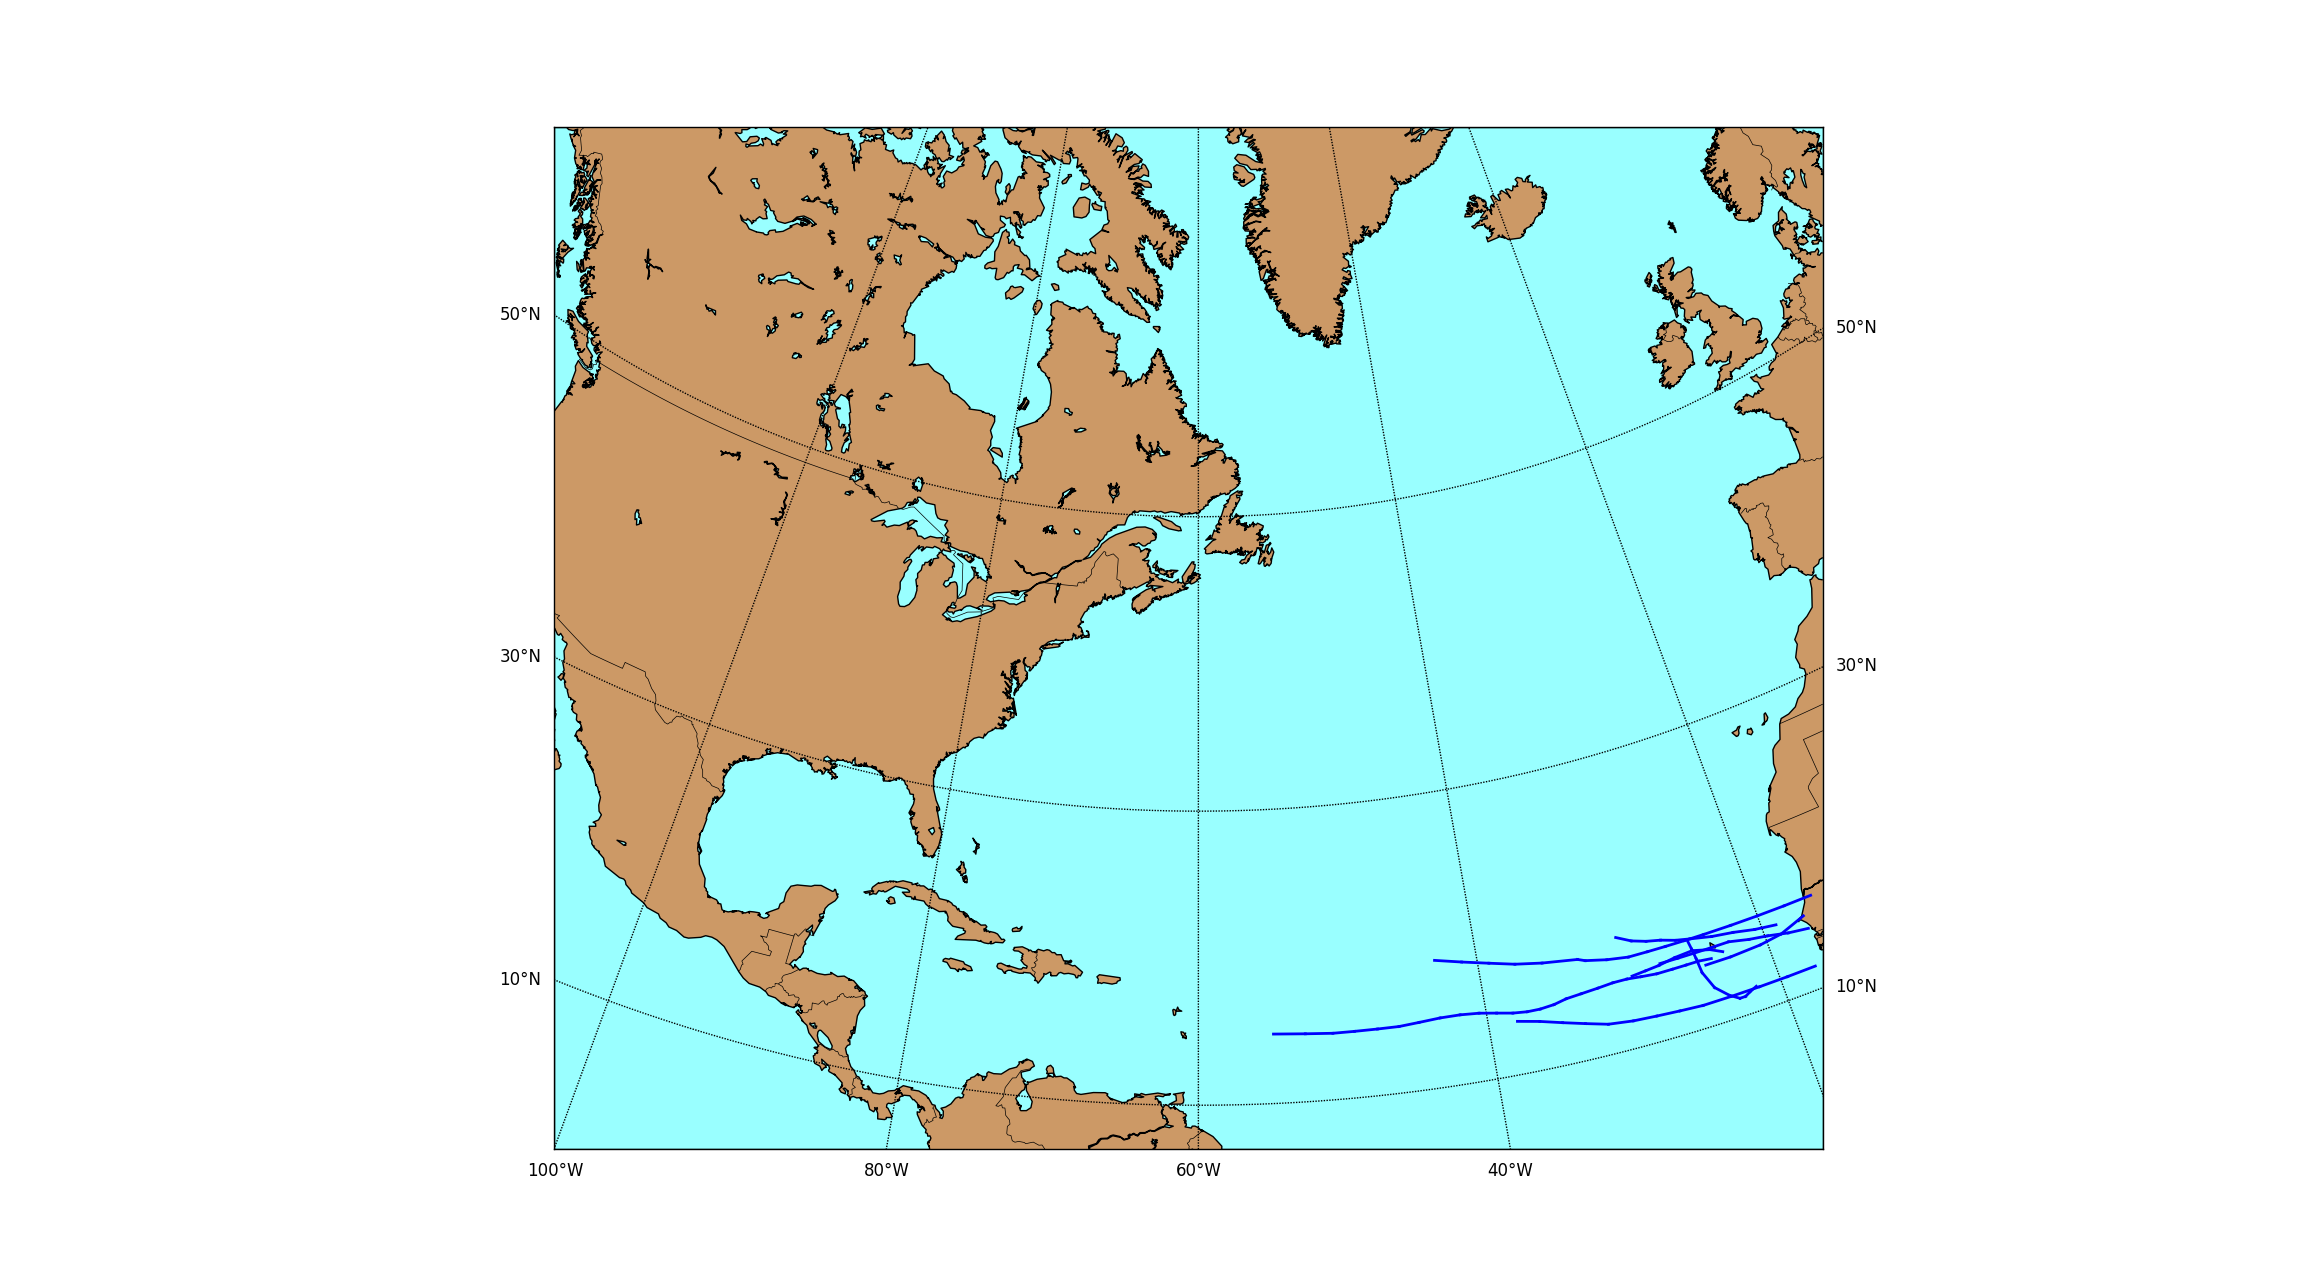
\includegraphics[width=\linewidth, trim=350 50 300 50, clip]{images/similar_hurricanes_4.png}
	\end{subfigure}
	\caption{The tracks from several sets of similar storms, according to the metric $M_{2}$. The red portion of the track is when the storm was hurricane strength, whereas the blue portion is when the winds were tropical storm force or lower. Qualitiatively, it's clear that the metric works as intended.}
	\label{fig:similar_hurricanes}
\end{figure*}

\subsection{Dimensionality Reduction}

\par
Now that I have a metric with which I can compare two hurricanes, compute a modified dissimilarity matrix $\mathcal{S}$ for hurricanes $H_{1},\ldots,H_{n}$
\begin{equation}
	[\mathcal{S}]_{i,j}=-\frac{1}{2}(M_{2}(H_{i},H_{j},\delta,\varepsilon))^{2}\;\;i,j\in\set{1,\ldots,n}
	\label{eq:dissimilarity}
\end{equation}
$M_{2}$, the $\SLC$ metric, is used because it is more effective than the $\LCSS$ metric according to \cite{ho2015manifold}.
In Figure~\ref{fig:similar_hurricanes}, I plot several sets of similar hurricanes to demonstrate the function of the metric.
Because $\SLC$ is a symmetric function, $\mathcal{S}$ is symmetric, so I only compute half of it and then reflect across the diagonal.

\par
I assume that there is some $k\in\N$ such that I can project our hurricanes into an $\R^{k}$ vector space, where the Euclidean distance between two hurricanes in $\R^{k}$ is approximately equal to their dissimilarity.
Let $P$ be this projection operator.
To compute the $P$, I use kernel principal component analysis (KPCA)~\cite{scholkopf1997kernel}, with $\mathcal{S}$ as a precomputed kernel.
This is implemented by~\cite{scikit-learn} in the python package \texttt{scikit-learn}.

\subsection{Kernel Regression}
In order to infer a relationship between the probability a storm makes landfall and its projection, I use Nardaraya-Watson kernel regression, presented jointly in papers by \cite{nadaraya1964estimating} and \cite{watson1964smooth}.
For $L$ the indicator random variable of whether or not a hurricane $H$ makes landfall, assume that $L=\mu(P(H))+e$ where $e$ is an error term and $E(e)=0$.
Let $H^{(i)}$ for $i=1,\ldots,n$ be the Hurricanes used to train the model, with $L^{(i)}$ whether or not each of them made landfall.
Then the Nardaraya-Watson estimator for kernel function $K$ and bandwidth $h$ is
\begin{equation}
	\hat\mu(P(H))=\frac{\displaystyle\sum_{i=1}^{n}K\paren{\frac{P(H^{(i)})-P(H)}{h}}L^{(i)}}{\displaystyle\sum_{i=1}^{n}K\paren{\frac{P(H^{(i)})-P(H)}{h}}}
	\label{eq:kernel_regression}
\end{equation}
Code to compute the estimator is implemented by \cite{seabold2010statsmodels} in the python package \texttt{statsmodels}.
I use a local linear regression, to mitigate bias issues at the edge of the support.

\subsection{Predicting Landfall}
Now that I have described the full model, I'll walk through the process of actually making a prediction for a new hurricane.
Let $H$ be a recently-formed hurricane or tropical storm (for our purposes, I assume at most $3$ days of track information).
First, I compute the dissimilarity $s_{i}$ with respect to each hurricane $H^{(i)}$, $i=1,\ldots,n$ in the training data sets in the same manner as Eq~(\ref{eq:dissimilarity}).
This gives us a vector $S$, which I can then project using our KPCA embedding to some vector $x=P(S)\in\R^{k}$. Finally, plugging $x$ into the Nardaraya-Watson estimator gives us some $y\in[0,1]$, which we take to be the probability that the hurricane will make landfall.